
This subsection provides brief descriptions of the parameterized simulations used to study 
the effects of model variations on the combination, and shows fit distributions comparing the 
simulations to those used in the experiments.  The simulation of each detector is referred to 
as the ``LHC-TeV MWWG'' or ``MWWG'' simulation for that detector.  A systematic uncertainty due to
the simplified parameterization is conservatively estimated by varying the lepton and recoil scales 
and resolutions by $\pm 5$\% and determining the effect on $\delta m_W$.

\subsubsection{CDF response and resolution model}

The CDF detector model consists of parameterizations of the electron and recoil momentum response 
and resolution.  The muon momentum response and resolution are similar to those of electrons. 

The electron fractional momentum resolution $\sigma_{p_{\tiny\textrm{T}}}/\pT = \sqrt{\kappa^2 + S^2/\pT}$ is modelled using
a sampling term of $S=12.6\%$~GeV$^{1/2}$ and a constant term of $\kappa=2\%$.  The constant term 
is larger than that used in the CDF simulation in order to correct for the lack of final-state radiation 
in the generated samples.  The leakage of the shower beyond the electromagnetic calorimeter is parameterized 
in the same manner as for the CDF measurement, and the reduction in electron momentum is corrected with a
scale factor applied to the electron momentum.

The recoil response is defined as the ratio $R(\pTW)$ of the measured recoil $u_T$ to the generated $\pTW$,
before accounting for effects of underlying event and additional proton-antiproton interactions (pileup).   
The CDF response is parameterized as 
\begin{equation}
R(\pTW) = r \log(a \pTW)/ \log(a \pT^{\scriptsize\textrm{ref}}),
\end{equation}

\noindent
where 
$r=0.65$, $a=6.7/$GeV, and $\pT^{\scriptsize\textrm{ref}} = 15$~GeV.  

The jet-like sampling for the recoil resolution is 
\begin{equation}
\sigma(\pTW) = s \sqrt{\pTW}, 
\end{equation}

\noindent
with 
$s=0.87$~GeV$^{1/2}$ and \pTW~in GeV. 
The recoil azimuthal angular resolution $\sigma_{u_\phi}$ is parameterized as 
\begin{equation}
\sigma_{u_\phi}(\pTW)  = \alpha - \beta \times \pTW,
\end{equation}

\noindent
where 
$\alpha=0.273$~rad and $\beta=0.016$~rad/GeV for $\pTW<\pT^{\scriptsize\textrm{ref}}$, and 
$\alpha=0.143$~rad and $\beta=0.0044$~rad/GeV for $\pTW \geq \pT^{\scriptsize\textrm{ref}}$.

The contribution of the underlying event to the measured recoil is represented by a randomly-oriented Gaussian 
distribution of width 
6.2~GeV.
Finally, the removal of lepton calorimeter towers from the recoil reconstruction is modelled by subtracting 660
MeV from the generated recoil along the direction of the decay lepton.

The distributions obtained using the MWWG simulation are compared with those from the CDF simulation 
in Fig.~\ref{fig:simuCDF}.  The agreement is at the percent 
level in the range of interest for the measurement.
The systematic uncertainties on the MWWG simulation are estimated by varying the response and resolution by $\pm 5\%$, 
calculating the $\delta m_W$ shifts for fourteen PDFs, and taking the maximum $|\delta m_W|$.  The resulting
uncertainties are 1.0 MeV for the \mT~fit, 0.9 MeV for the \pTl~fit, and 2.0 MeV for the \met~fit.
 
 \begin{figure}[!tbp]
   \centering
   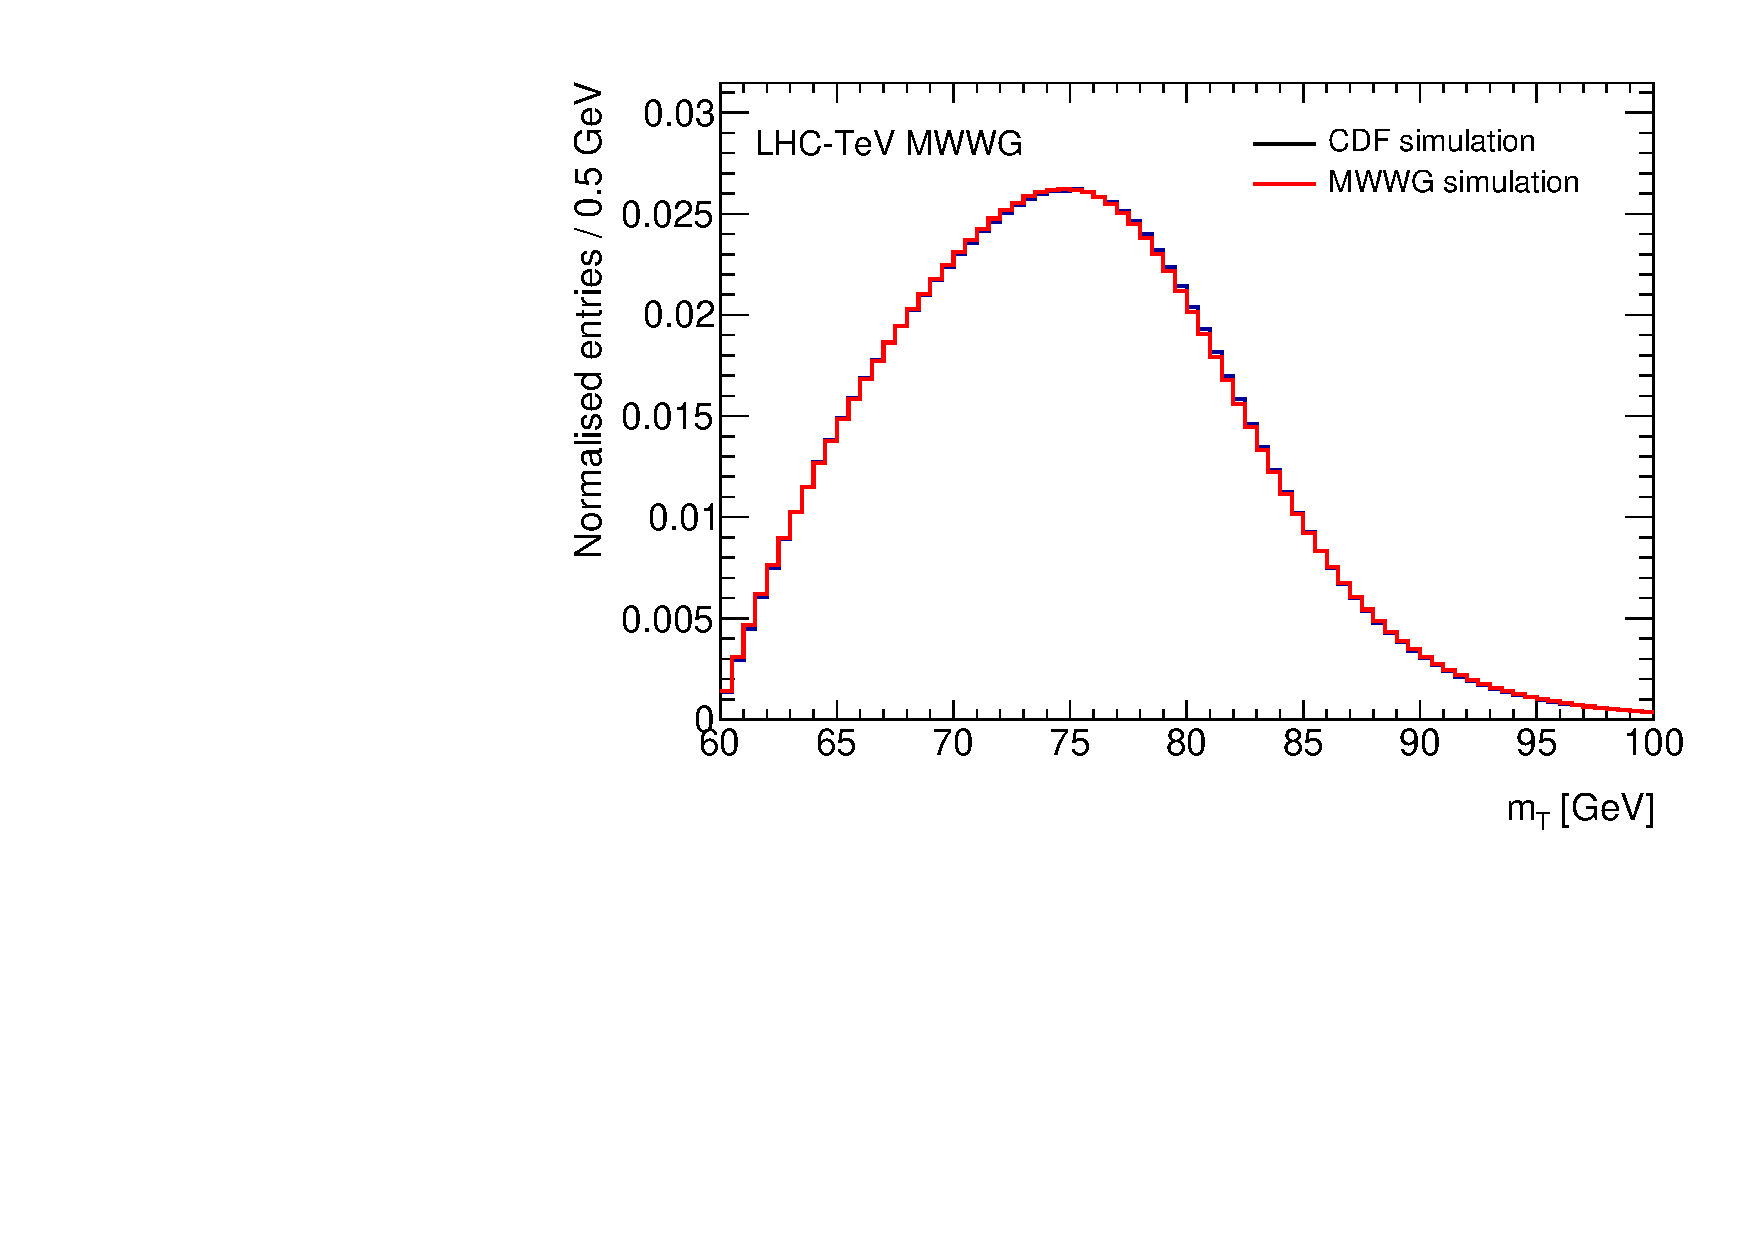
\includegraphics[width=0.98\columnwidth]{Wmt_data_fit_norm_overlay.pdf}
   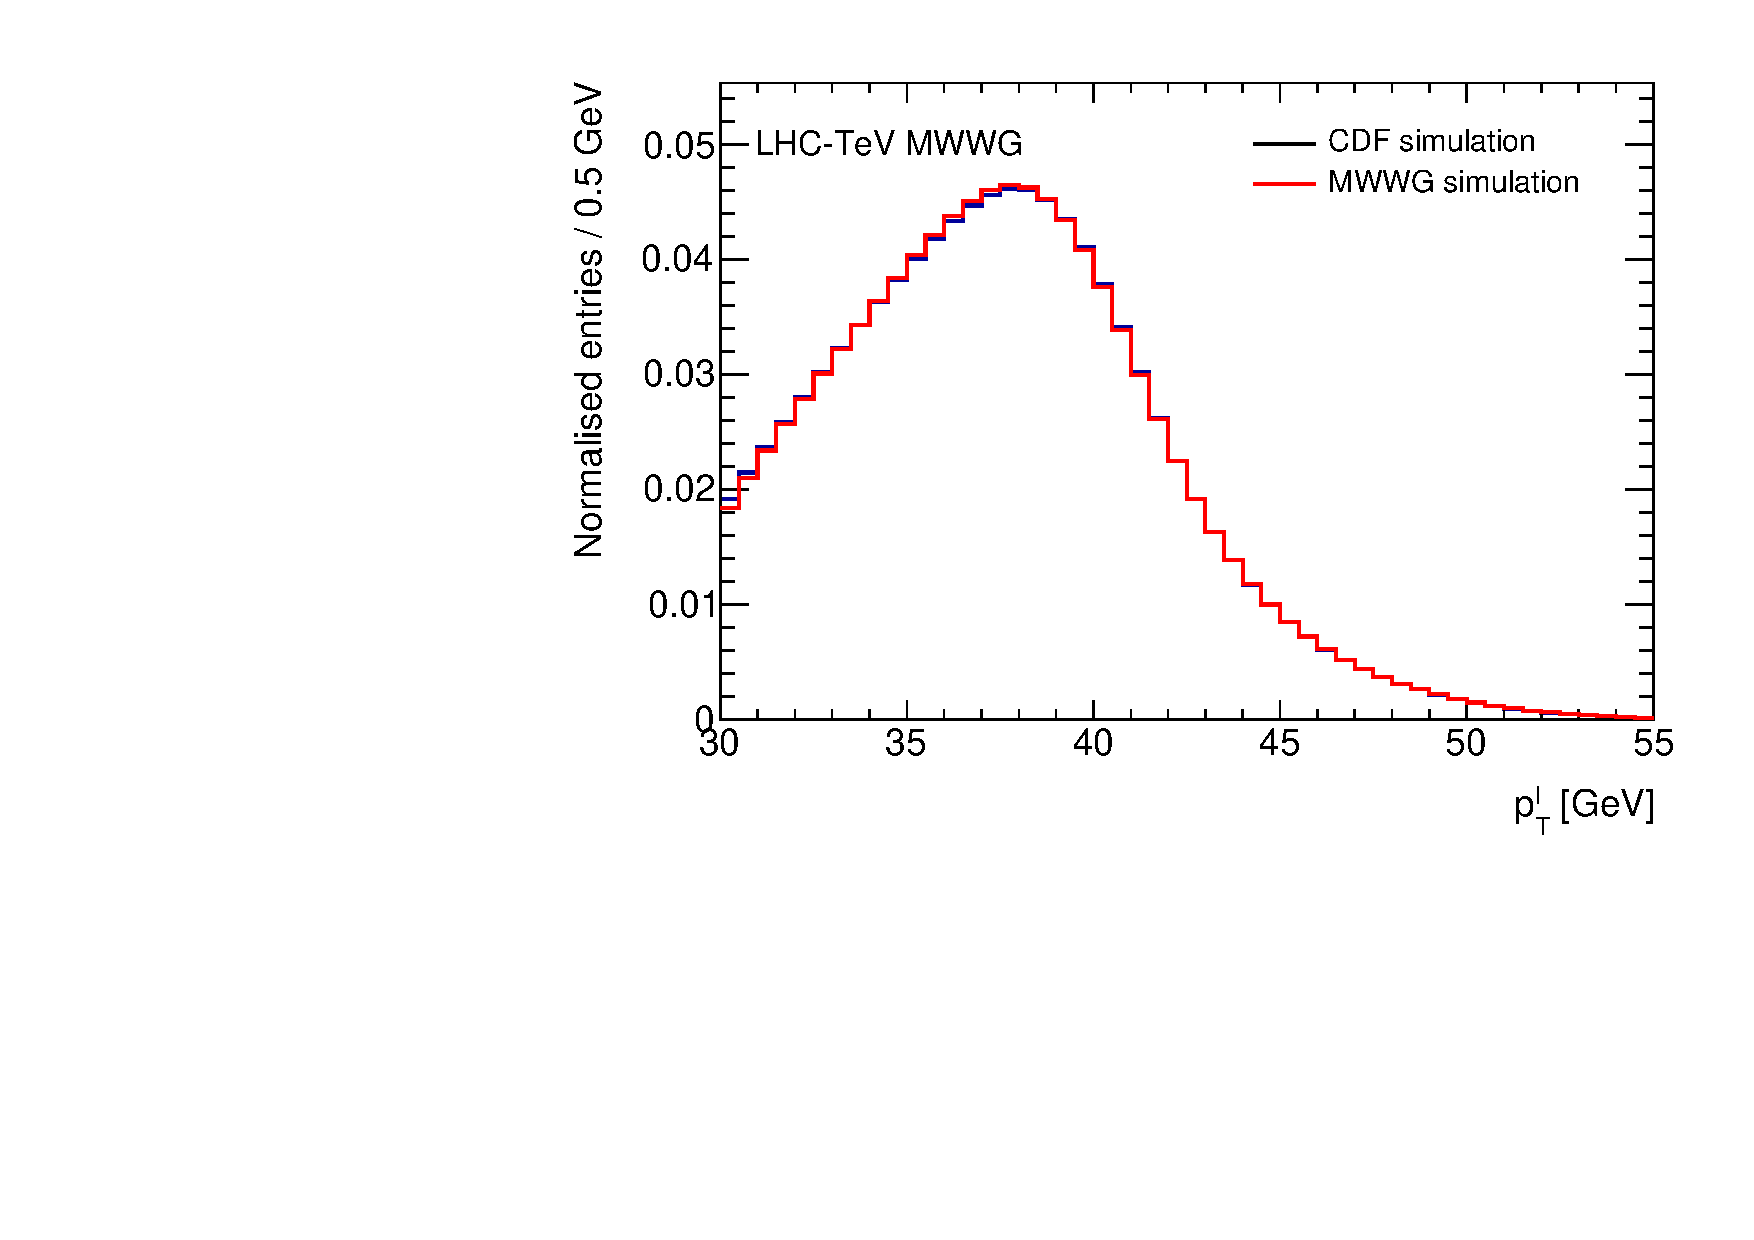
\includegraphics[width=0.98\columnwidth]{Wpt_data_fit_norm_overlay.pdf}
   \caption{
Comparisons between the CDF simulation~\cite{Aaltonen:2013vwa} and the LHC-TeV MWWG simulation for 
the \mT~(top) and \pTl~(bottom) distributions.  
}
\label{fig:simuCDF}
\end{figure}


\subsubsection{D0 response and resolution model}

The LHC-TeV MWWG simulation of the D0 detector includes a model of the efficiency of the electron reconstruction and 
selection along with the response and resolution of the recoil and the electron momentum.  The simulation reproduces 
distributions from the D0 parameterized Monte Carlo simulation (PMCS) used for the final D0 measurement based on an 
integrated luminosity of 4.3~\ifb{}~\cite{D0:2013jba}.  The prior measurement based on 1.1~\ifb{}~\cite{Abazov:2009cp} 
of integrated luminosity has a lower mean number of pileup events; the corresponding impact on the estimation of
mass shifts is within the applied uncertainty.

The electron energy response is parameterised as:
\begin{equation}
E = \alpha(E_0-\bar{E_0}) + \beta + \bar{E_0},
\end{equation}
where $E$ is the calibrated electron energy, $\bar{E_0}=43$~GeV is a reference value corresponding to the electron energy 
in $Z$-boson events, and $\alpha$ and $\beta$ are luminosity-dependent energy scale and offset corrections, respectively.  
We take $\alpha=1.0164$ and $\beta=0.188$~GeV, the values determined in Ref.~\cite{D0:2013jba} for an instantaneous 
luminosity in the range (2--4)$\times 36\times 10^{30}$\instlum~corresponding to the largest fraction of the 
data.  Implementing the instantaneous luminosity dependence gives results in agreement with the average response to 
within a percent.

The electron energy resolution $\sigma_E/E$ is simulated using the same functional form as for CDF, with a constant term
of $\kappa=1.997\%$~\cite{D0:2013jba} and a sampling term of
\begin{eqnarray}
  S &=& S_0 \exp\left[S_1\left( \frac {1}{\sin\theta}-1\right)\right] + \frac{S_2\eta+S_3}{\sqrt{E}},
 \end{eqnarray}
where $S_0=0.153$~GeV$^{1/2}$, $S_1=1.543$, $S_2=-0.025$~GeV, $S_3=0.172$~GeV, and $E$ is in GeV. The resulting fractional
resolution is increased by 2\% to account for the lack of generated final-state radiation and improve the agreement with the
distributions from the D0 PMCS.

The electron reconstruction and identification efficiency is modeled by the following function
determined using the data points in Fig.~25(b) of Ref.~\cite{D0:2013jba}:
\begin{eqnarray}
\varepsilon( \pTl)&=& 0.95 \left(1- e^{-{0.074  \pTl}}\right),
\end{eqnarray}
where \pTl~is in GeV.

The recoil is modelled using a migration matrix to obtain a simulated \uT~value for a given generated
\pTW~\cite{D0:2020ujb}.  In order to model the recoil energy in the electron cone that is not included
in the recoil measurement, 150~MeV are subtracted from the recoil component parallel to the decay
lepton~\cite{D0:2013jba}.

Figure~\ref{fig:simuD0} shows the \pTl~and \mT~distributions from the D0 PMCS and the LHC-TeV MWWG 
simulation after reweighting the events to match the \pTW~distribution used for the D0 measurement.  The distributions
agree to within 2\% in the range of interest for the $m_W$ extraction.  The shifts in $m_W$ are studied for the 
eigenvectors of the CTEQ6.6 and CT10 PDFs, and the MWWG simulation and D0 PMCS agree within the statistical 
precision of $\approx 1$~MeV.  Systematic uncertainties are determined by varying the scales and resolutions, and 
calculating the effect on $\delta m_W$ for fourteen PDF sets.  The resulting uncertainties are 1.0 MeV on the \mT~fit, 
1.0 MeV on the \pTl~fits, and 2.2 MeV on the \met~fit.

\begin{figure}[!tbp]
  \centering
  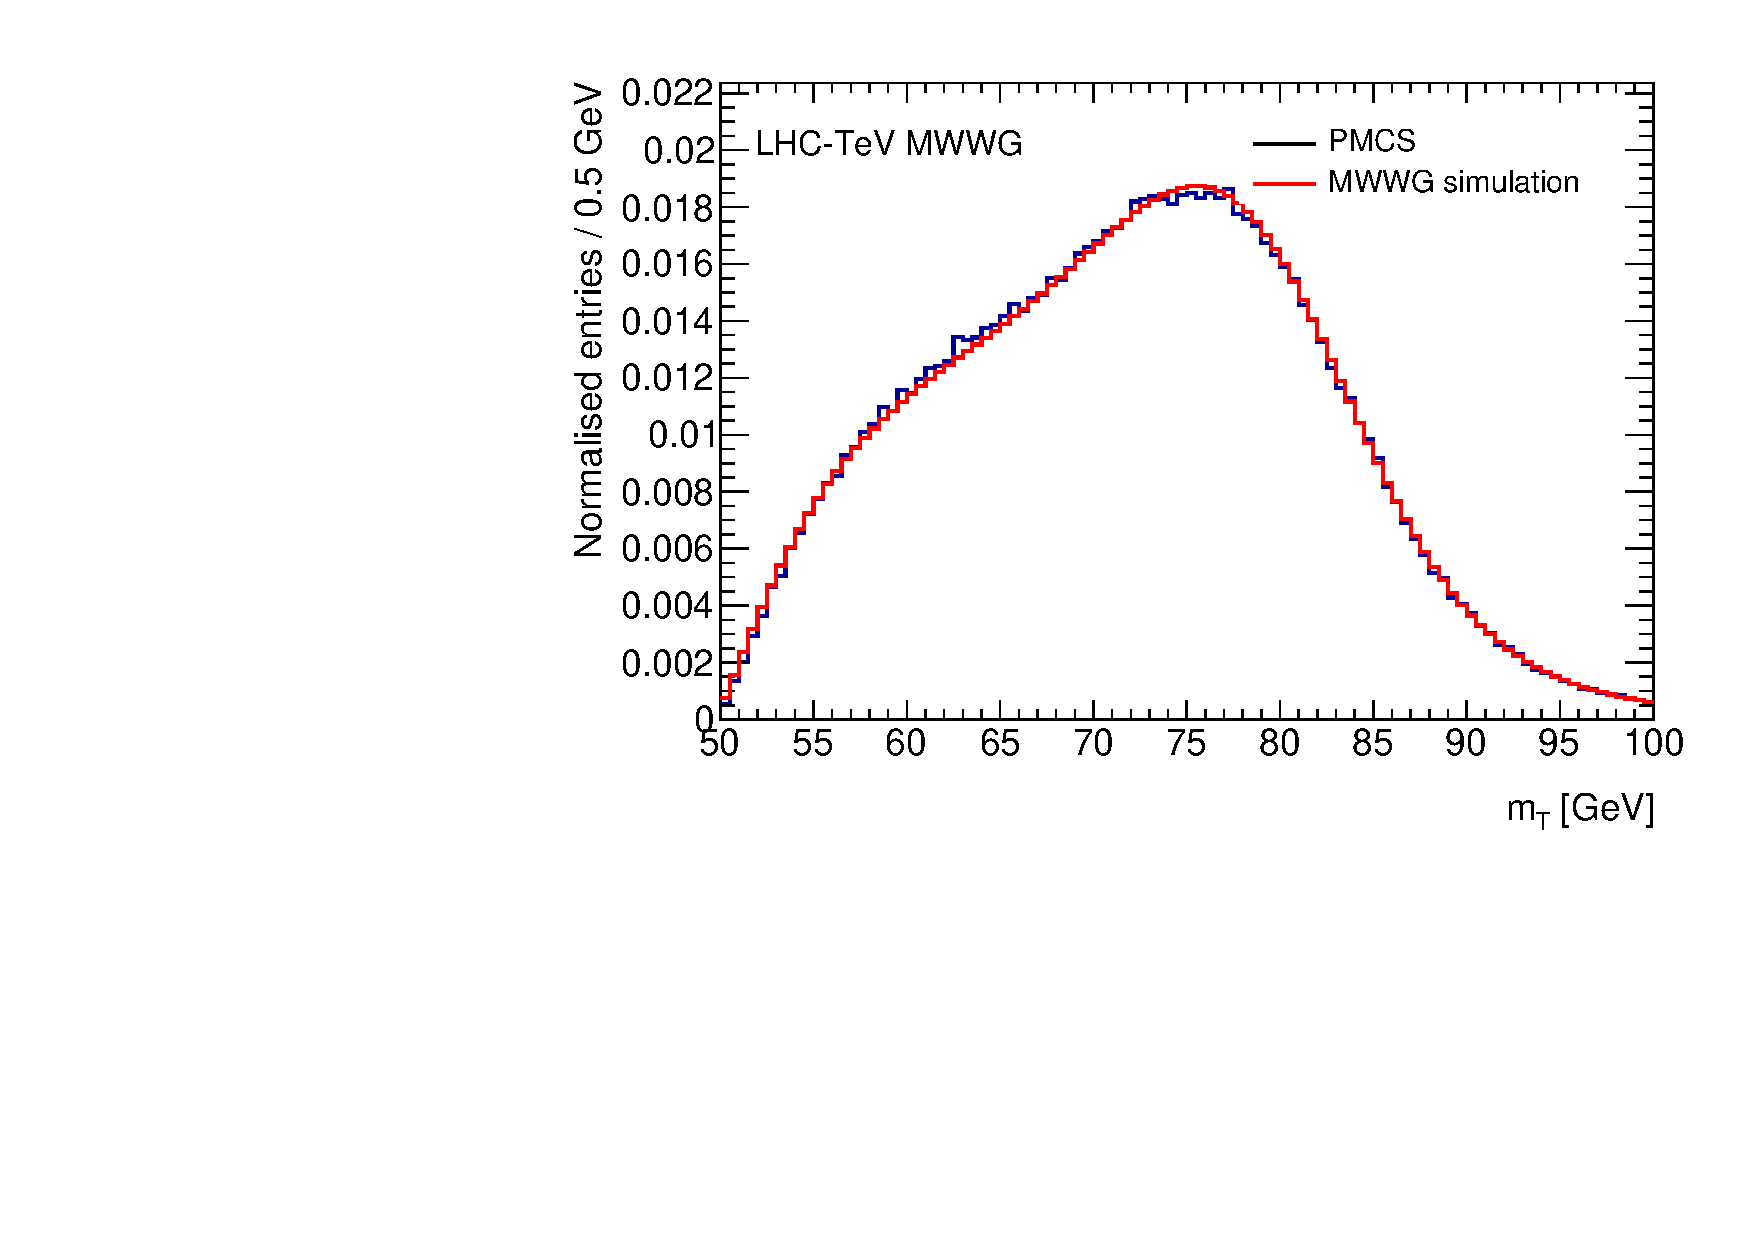
\includegraphics[width=0.98\columnwidth]{MT_MC_norm_overlay.pdf}
  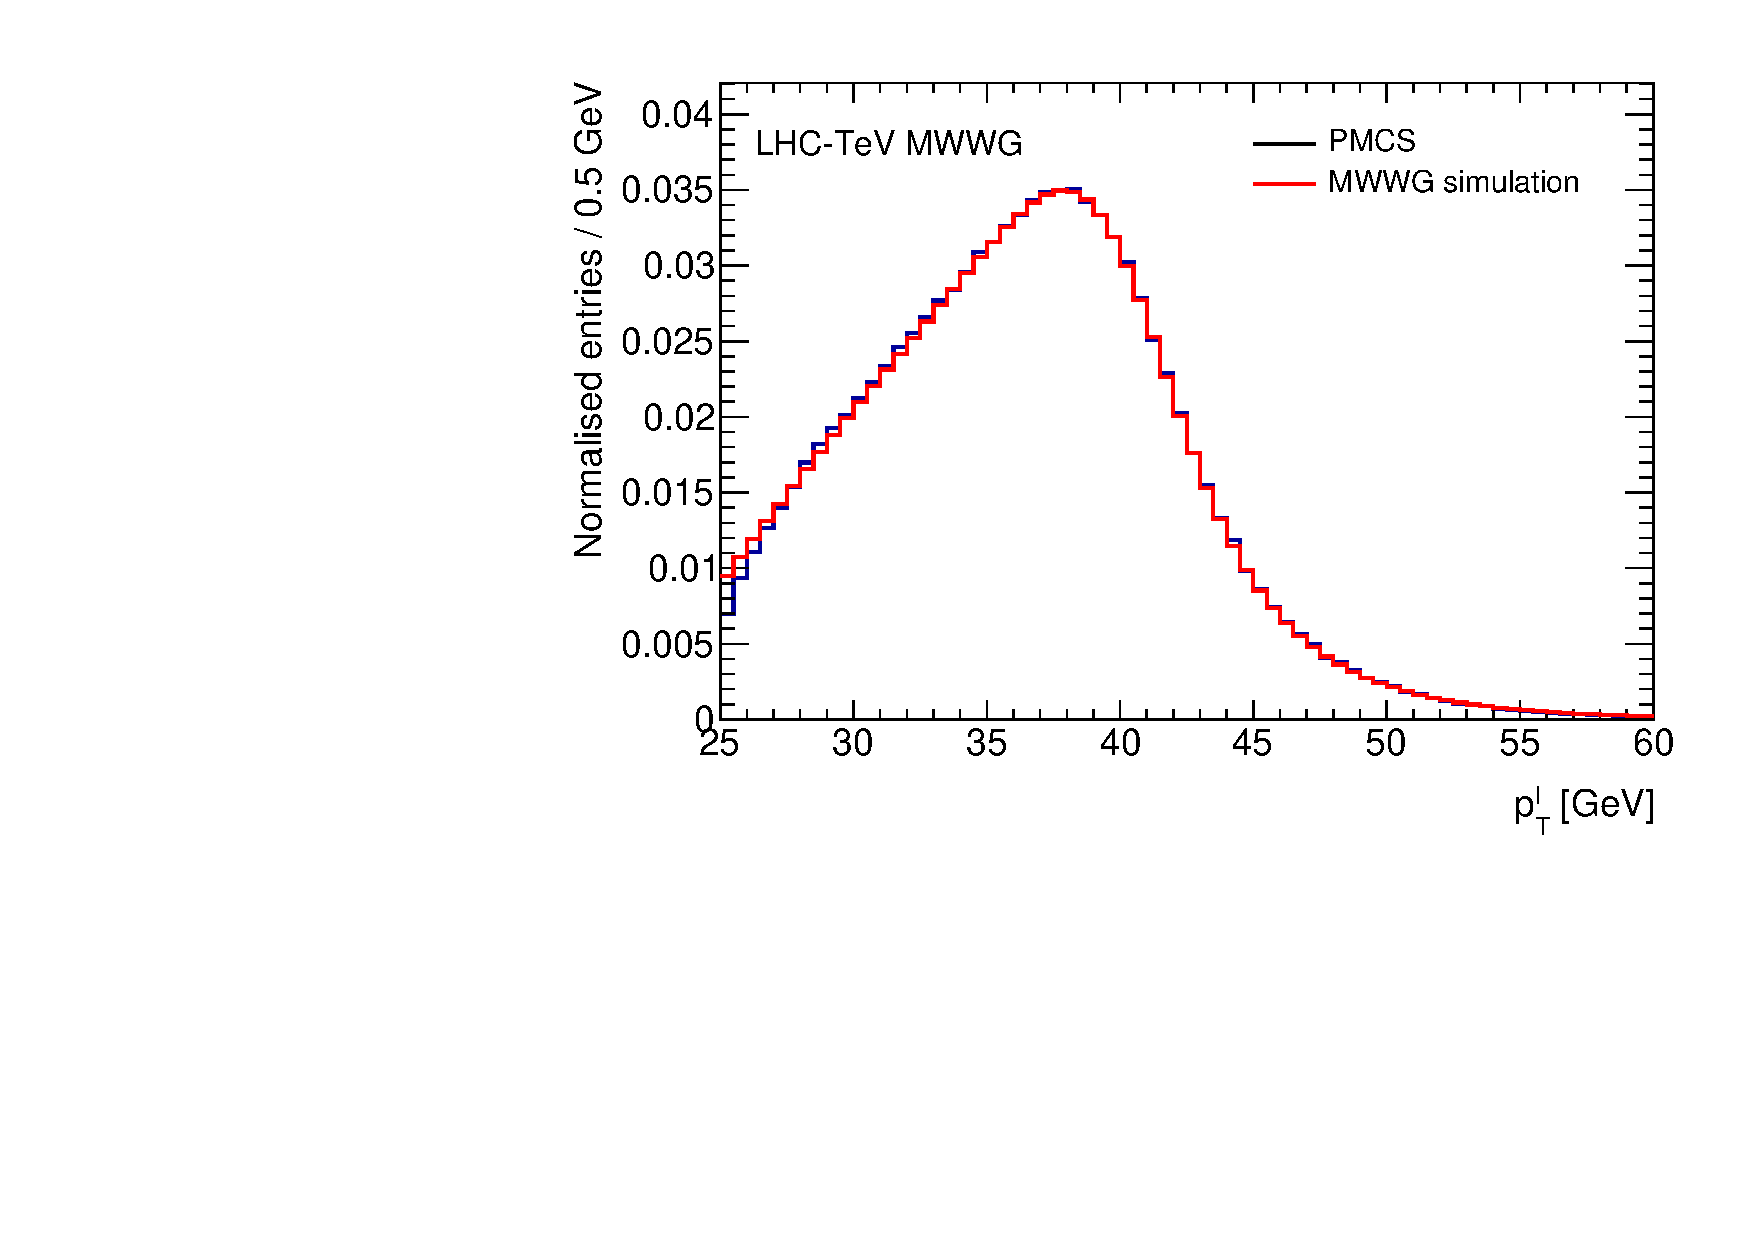
\includegraphics[width=0.98\columnwidth]{ElectronPt_MC_norm_overlay.pdf}
  \caption{Comparisons of the D0 PMCS and the LHC-TeV MWWG simulation for the \mT~(top) and \pTl (bottom) distributions. 
}
\label{fig:simuD0}
\end{figure}


\subsubsection{ATLAS response and resolution model}

The ATLAS recoil response and resolution are parametrized using distributions~\cite{Aaboud:2017svj} of the projections
of these quantities
along and perpendicular to the lepton direction, as a function of the $W$-boson transverse momentum.  The parameterizations
are calibrated using the full ATLAS simulation.  The recoil resolution ranges from 12 to 16~GeV, depending primarily
on the amount of pileup.  
The electron and muon resolutions are parameterized using the documented detector performance~\cite{PERF-2013-05,PERF-2014-05}.
The resulting \pTl~and \mT~distributions are given in Figure~\ref{fig:simuATLAS}, which shows that the resolution is
accurately modeled and that residual differences could be improved with lepton energy scale adjustments and do not
significantly affect the results.

\begin{figure}[!tbp]
  \centering
%  \includegraphics[width=0.98\columnwidth]{pTl_plmunu_ATLAS.pdf}
%  \includegraphics[width=0.98\columnwidth]{mT_plmunu_ATLAS.pdf}
  \includegraphics[width=0.98\columnwidth]{atlas_pTl.pdf}
  \includegraphics[width=0.98\columnwidth]{atlas_mT.pdf}
  \caption{Comparison of the published and MWWG simulated \pTl~(top) and \mT~(bottom) distributions for ATLAS.
%\textcolor{red}{FINAL PLOTS NEEDED WITH MC REPLACED BY SIMULATION AND EMULATED REPLACED BY MWWG.}
%\tcr{Update these plots ($\to$ Maarten)}\label{fig:simuATLAS}
% add ratio panels below?
}
\label{fig:simuATLAS}
\end{figure}

The accuracy of the LHC-TeV MWWG simulation in determining $m_W$ shifts is studied using PDF variations from the 
ATLAS measurement.  With 28 measurement categories and 25 CT10 PDF eigensets, a statistically accurate comparison 
is made between the emulated measurement procedure and the results of the ATLAS measurement.  
%Figure~\ref{fig:shifts2} shows 
%the results of this comparison with $\delta m_W$ as defined in Sec.~\ref{sec:methods}, where the reference set is the 
%CT10nnlo central set and the variations are the corresponding uncertainty sets.  
A root-mean-square spread of 1.5 MeV is found between the published and emulated shifts in the various categories and eigensets.
The differences dominantly reflect approximations in the {\textsc{Powheg}}-based reweighting procedure compared to the
kinematic reweighting to NNLO-accurate distributions implemented in Ref.~\cite{Aaboud:2017svj}.
%Similar variations are
%observed when using the procedures used to estimate the systematic uncertainties on the MWWG simulations of the D0
%and CDF detectors.
Systematic uncertainties are assessed by varying the response and resolution by $\pm 5\%$, and are 1.1 MeV for the
\pTl~fit and 1.2 MeV for the \mT~fit.
